% \glsresetall
\chapter{Content Delivery Networks} % Main chapter title
\label{Chapter3}

\lhead{Chapter 3. \emph{Content Delivery Networks}}

This chapter will give further information about the CDN technology and how it was implemented for the context of this thesis.

\section{CDNs in general}

CDNs are commonly used on the Internet these days. This is due to the fact that CDNs have become a convenient way of providing the resources a website needs in split seconds, thus increasing its performance and the overall user experience.\cite{cdn_general}
The following sections will provide an overview of the CDN technology.

\subsection{Architecture}

The basic architecture of a CDN can be split into three different building blocks.

\begin{itemize}
	\item \textbf{Point of Presence (PoPs)} - Strategically located data centers around the world. Their function is to reduce the round trip time of requests. PoPs usually consist of several caching servers.
	\item \textbf{Caching servers} - These servers are located in different PoPs and serve the function of caching resources from the origin server. That way website loading times and bandwidth allocations are reduced.
	\item \textbf{Hardware, like SSD/HDD and RAM} - Located in the cache servers, the purpose of this building block is to provide the necessary storage and computing capacity. Better hardware means faster computing time, which then again improves the overall performance of the designated caching server.
\end{itemize}

Besides the above three building blocks, another one is crucial for the architecture of a CDN: The \textbf{origin server}. In a CDNs topology, the origin server can be compared to the center, or core. This is the server onto which the CDNs content is uploaded, synced with or distributed over the CDNs caching servers.\cite{cdn_origin_server}

An example for a basic CDN distribution is shown in figure \ref{fig:cdn_general_arch}.

\begin{figure}[!h]
	\centering
	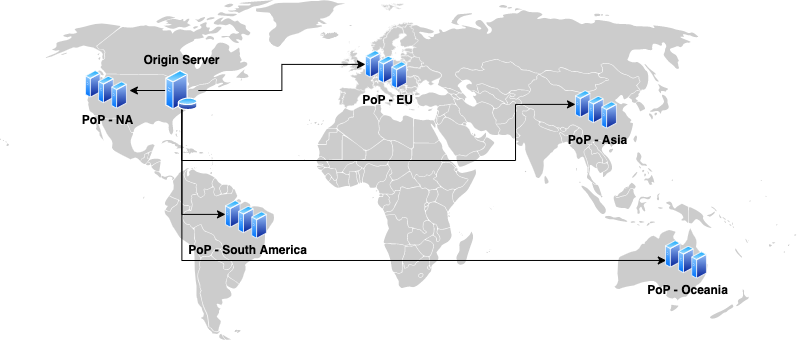
\includegraphics[width=1\textwidth]{Figures/basic_cdn_arch.drawio.png}
	\caption{Basic distribution a CDN}
	\label{fig:cdn_general_arch}
\end{figure}

It has to be mentioned that the geographical distribution in figure \ref{fig:cdn_general_arch} is simplified, for the sake of readability. In a real scenario, the cache servers of each PoP would themselves be distributed over different data centers on the continent. A client requesting resources from the CDN always communicates with the nearest cache server to their designated location.\cite{cdn_general}

\subsection{Design}

For a CDN to fulfill its purpose, four requirements have to be met. These are not only technical requirements, like necessary hardware, but rather concerning the general design of the CDN.
The four pillars of CDN design are:

\begin{itemize}
	\item \textbf{Performance} - First and foremost, the CDN has to provide a benefit when it comes to website performance. When the usage of a CDN increases the loading time of a website, the negative effect on user experience can cause financial harm to the host.\cite{cdn_general}
	\item \textbf{Scalability} - Since a cache server can serve multiple resources to different websites, it has to be able to handle traffic peaks. Without the aspect of scalability (either horizontal or vertical), these requirements cannot be met which would affect the CDNs performance.
	\item \textbf{Reliability} -  A website host has to rely on the CDN to deliver the websites resources. An outage on CDN side would cause the same effect to the relying websites, resulting in additional costs for the designated hosts. Therefore, CDN providers commit to 99.9\% service level agreements (SLAs).
	\item \textbf{Responsiveness} -  The aspect of responsiveness targets the issue of synchronization inside the CDN. A CDN has to be capable to react to changes and distribute those to its PoPs over the globe accordingly. Otherwise inconsistencies could occur on the websites relying on the CDN. This is ensured through an automated pull mechanism, via which edge servers pull changes from the origin server.\cite{cdn_origin_server}
\end{itemize}

Additionally to those four requirements, the topology of a CDN has to be considered. There are two options which can be used. Both would serve their purpose, but have different advantages as well as disadvantages. 

\begin{itemize}
	\item \textbf{The scattered CDN} - This topology focuses on physical proximity. The PoPs are kept rather small in size, but are scattered around the world in greater frequency, thus providing as much proximity to their client as possible. This topology excels in providing the CDN's resources into low-connectivity regions, since it is not highly dependent on wire infrastructure. When it comes to latency, it does not suffer as much due to the short distance between client and server. The trade-off with this topology is that it accrues more maintenance costs, since more PoPs are required to be maintained. Also, deploying new configurations can be connected to a lot of effort, depending on the number of PoPs scattered across the CDN. 
	Additionally, this number can also affect the RTT since every PoP inbetween the client and the server is a connection point.
	
	\item \textbf{The consolidated CDN} - Contrary to the scattered CDN, this topology is designed to consolidate its resources at strategically located data centers. Since the PoPs are only located in those major data centers, the servers available to the PoPs are highly advanced and provide a lot of hardware capacity. Additionally, since the number of major data centers around the world is rather limited, the number of PoPs is reduced as well, compared to the scattered topology. Following the quality over quantity principle, a PoP in this topology can handle a greater amount of traffic compared to its counterpart, and is also more resilient, specifically when it comes to DDoS attacks. Also, due to the moderate number of PoPs, it is easier and faster for the operators of the CDN to deploy new configurations.
	Nonetheless, the trade-off for this topology is that, even though it can handle a high number of requests, its reach to low-connectivity regions is rather limited. This is due to the proximity difference between the servers and clients. Additionally, deploying a new PoP into this topology requires more effort, since the PoPs are rather complex.	
\end{itemize}

The design decision is of course dependent on the business case for the CDN, as both topologies are intended to solve specific issues or challenges. \cite{cdn_architecture} 

\subsection{Optimization}

The CDN technology offers several ways of optimizing a websites performance and therefore, improving the user experience. In the following section these optimizations will be showcased and explained.

\subsubsection{Route optimization with Anycast}

As previously mentioned, a CDN can be designed with different topologies which can affect its performance. Another factor which has to be considered in this equation is the routing itself. Basically, it does not matter if a cache server is located in close proximity to a client, if the requested resource is not present there. In this case, the client would have to be routed to different, cache servers located further away. 
To circumvent this, the Anycast routing is used in modern CDNs. This traffic routing algorithm is best explained in direct comparison with Unicast. Both serve the same purpose of routing requests to their designated destination, but they do it in different ways. Where with Unicast each node has a unique address, Anycast advertises multiple nodes with the same address.
For instance, in a Unicast orchestrated network the server address \texttt{10.10.0.1} would be only present once. Anycast, on the other hand, would advertise this exact address over multiple different servers around the globe. Thus, a request towards the address would reach its destination via the shortest path, given that the path will be identified and prioritized by devices that actually govern the flow of traffic.
The shortest path itself is counted in hops. Hops represent the number of time a request changes hands between hosts.\cite{cdn_route_opt}

\subsubsection{TLS Performance}

The route optimization with Anycast, also improves the RTT when using the TLS/SSL protocol. Since this section does not focus on explaining the protocol, only a short description is given.
SSL (Secure Socket Layer) or, as it now should be called, TLS (Transport Layer Security) is a protocol via which secure communications are ensured on the Internet. The communicating parties establish a connection via the following steps:

\begin{enumerate}[noitemsep]
	\item A so-called three-way handshake is done
	\item The parties agree upon an encryption method
	\item Mutual verification process is performed
	\item Symmetric keys for encoding and decoding are generated
\end{enumerate}

These steps are necessary to ensure secure communication and are a welcome trade-off for the benefits they provide. 

A CDN can provide improvement to this overhead and decrease the RTT of a request. Through the aspect of route optimization and general proximity, the overall request distance is decreased. Therefore, the RTT is shortened as well. The steps are still processed, they just do not have to travel that long. Additionally, the SSL/TLS negotiation process is shorter, too.\cite{cdn_ssl_tsl}

\subsubsection{Frontend optimization}

The term frontend optimization refers to the process of making a website more browser-friendly and reducing loading times. There are multiple ways to optimize a frontend. These will be explained under consideration of the role a CDN plays in them.

\begin{itemize}
	\item \textbf{Reducing HTTP requests} - When loading a website, the browser opens several HTTP connections, the number of which is actually limited by the browser. If a website requires more connections than a browser can open at the time, the browser has to start queuing the rest. This again leads to longer loading times and affects the user experience. A CDN improves on that by pre-pooling connections and ensuring they remain open throughout a session. Even though this does not reduce the actual number of requests, it does improve the response time for each one, making it so that every request can be processed faster. Additionally, HTTP/2 introduces the method of multiplexing. This allows a single TCP connection to transfer multiple different HTTP requests \cite{http2}.
	
	\item \textbf{File compression} - Of course it is not always about the number of requests per site or the proximity of the client to the server. The actual content does affect the responsiveness, too. Loading one single resource with a size of 1 GB takes a while, even if the server is close by. Reducing the size of this file or resource might increase the loading process. File compression like gzip is a method of doing exactly that. Most modern CDN providers offer automated file compression with gzip to reduce the actual content size delivered to the client.
	
	\item \textbf{Cache optimization} - Via caching, static files are stored either on the client device or in the cache of a nearby cache server. Locally stored static files do not have to be loaded via the network and are available to the browser for rendering almost immediately. The only question remaining is how long does a resource have to be cached. This information is necessary to optimize the use of the client's cache. The caching time is usually defined in the cache header of the request. Modern CDNs offer cache control options, which help in defining rules for exactly that header.
	CDNs have also started to use machine learning techniques to follow and understand content usage patterns and automatically optimize caching policies.
	 
	\item \textbf{Code minification} - Similar to the file compression method, the process of code minification offers a way of reducing file sizes too. Whereas a developer writes code in a humanly readable way, with spaces and line breaks, a machine does not need this kind of formatting. By removing comments, spaces and line breaks, the size of a code file can be reduced by 30\%. CDNs use methods like gzip, minify or a combination of these two to reduce the size of JavaScript, HTML or CSS files.
	
	\item \textbf{Image optimization} - Images can be immense in size and require a long time to load. The best way to display an image on a website would be to cache it first and then load it from the cache to reduce actual loading time through the network. Another option could be to reduce the actual size of the image and thus the loading time.
	However, other than code files, images are already compressed when loaded, therefore compressing them further to reduce file size might cause a loss of image quality. This is called lossy compression. If this trade-off is not an option, caching would be more effective.
	CDNs offer exactly that solution, caching images and providing them from the nearest source available to the client. If this does not suffice, CDNs also offer a progressive rendering option for images. On initially loading the page, the CDN would provide a lossy compressed version of the image quickly and then progressively replace it with higher-resolution variants.
	Alternatively, a website host could use vector or raster images. These are resolution independent, smaller in size and highly responsive.\cite{cdn_fe_opt_img_opt}
\end{itemize}

These methods in combination with the CDN technology provide a possible gain in user experience for a website host. \cite{cdn_fe_opt}
\section{Unpkg}

As described in \ref{cdn_intro}, the concept of CDN is fairly simple. A remote server is providing the necessary platform resources via an API, thus avoiding the necessity of bundling those resources.
To evaluate the impact of this technology on a micro frontend landscape, a prototype was developed using the public cloud based CDN Unpkg.com.
%\begin{figure}[!h]
%	\centering
%	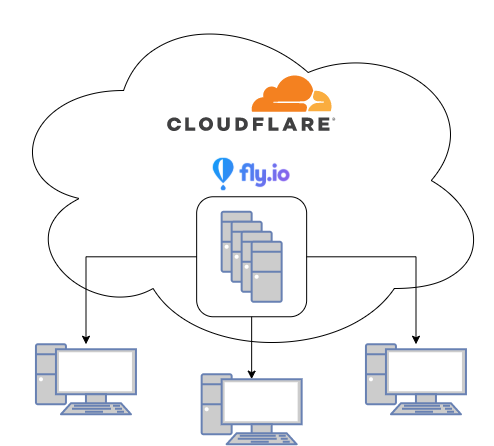
\includegraphics[width=0.7\textwidth]{Figures/cdn_unpkg.drawio.png}
%	\caption{Basic architecture of the unpkg.com public CDN}
%	\label{fig:unpkg_architecture}
%\end{figure}

%Figure \ref{fig:unpkg_architecture} shows the Unpkg.com architecture, as it is described in its official documentation. 
It is an open-source project, built and maintained by Michael Jackson. It runs on the Cloudflare platform, and auto-scalable servers are provided by Fly.io, which are located in 17 cities around the world.\cite{unpkg_doc}

An open API is available, through which resources can be requested. Via path and query parameters in the URL, necessary information like the dependency version can be provided.

The previously mentioned prototype was developed using Unpkg.com. Figure \ref{fig:unpkg_prototype_architecture} visualizes the architecture of the prototype.

\begin{figure}[!h]
	\centering
	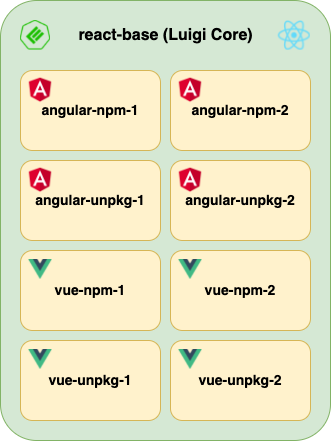
\includegraphics[width=0.7\textwidth]{Figures/unpkg.architecture.drawio.png}
	\caption{Architecture of the Luigi prototype using unpkg.com}
	\label{fig:unpkg_prototype_architecture}
\end{figure}
\newpage
Several Nodes were embedded in the Luigi landscape, some of which are Angular apps, other are implemented with Vue. It has to be noted, that apart from the difference regarding the UI-Frameworks, each micro frontend displays the same elements. This design decision was made to ensure a base for later comparisons. Additionally, each micro frontend was implemented using a regular bundler and package manager. This way, a direct comparison is possible between the two technologies.

The usage of the Unpkg-CDN itself is embedded in the code. Instead of loading the dependencies via the local \texttt{node\_modules} directory, they are directly loaded using the CDNs API, the usage of which is displayed in the listing \ref{unpkg_import}.

\begin{lstlisting}[caption=Import of a dependecy using the unpkg API, label=list:unpkg_import]
	<script src="https://unpkg.com/@ui5/webcomponents@1.0.0-rc.15/dist/StandardListItem.js?module" type="module"></script>
\end{lstlisting}

This script tag is placed in the central \texttt{index.html}. The loaded resource can be read from the URL. The first part of the URL refers to the protocol and the host. The first path parameter is the npm dependency name. In the case of \ref{unpkg_import} it is \texttt{@ui5}, followed by a subdirectory with its respective version annotated with an @.
As it is described in the documentation, the CDN supports two query parameters.

\begin{itemize}[noitemsep]
	\item \texttt{?meta} - to request meta data about the loaded package, in a JSON format
	\item \texttt{?module} - to expand all import specifiers in JavaScript modules to unpkg URLs
\end{itemize}

If the import is handled via a script tag, as it is done in \ref{unpkg_import}, the \texttt{type="module"} attribute has to be added, depending on the resource loaded.
In the case of the given example, the resource is a JavaScript module type. To ensure it is parsed by the runtime as such, this attribute has to be added.\cite{js_module_type}

\section{Owning a CDN}

Even though the method of a self-hosted CDN was not implemented in the developed prototype, it has to be considered for the context of this thesis. Since the basic principle of a CDN was already explained, this section will focus on the financial aspect of the technology.

This topic will be showcased based on a hypothetical scenario. The numbers and metrics of this scenario are either assumed or taken directly from the implemented prototype.

The first requirements of the scenario are the following:

\begin{itemize}[noitemsep]
	\item A micro frontend landscape has to be developed. 
	\item To reduce the runtime costs, the loading of redundant libraries should be avoided in the landscape.
	\item The libraries for the landscape were developed by the same team and are only available for internal use.
\end{itemize} 

These circumstances ensure that only a self-hosted CDN is applicable.
Next, the numbers and further requirements of the landscape are necessary. Those are required for the cost calculation of the CDN.
It is mentioned if the numbers are actually \textit{assumed/estimated} or \textit{taken from the prototype}.

\begin{itemize}[noitemsep]
	\item How often the site is accessed per day - $50 000$ times (estimated)
	\item Avg. byte size per page load without caching on client side - $8983.5$ KB (taken from the prototype)
	\item Avg. amount of GET requests to CDN per site load - $198$ requests (taken from the prototype)
	\item The site is only accessed in North America 
\end{itemize} 

Based on those requirements, the following values are calculated for the monthly CDN usage of the described scenario landscape.

\begin{quote}
	\begin{center}
		Let $A$ be the amount of requests to the CDN per month:
		\begin{math}
			A = 50000 \times 30 \times 198 = 297000000
		\end{math}
	\end{center} 
\end{quote}

\begin{quote}
	\begin{center}
		Let $B$ be the amount of bytes loaded per month:
		\begin{math}
			B = 50000 \times 30 \times 8983.5 = 13475250000 \: $KB$ \; = 13.47525 \: $TB$
		\end{math}
	\end{center} 
\end{quote}

In the following text, it will be analyzed how much it would cost a company or department to pay for the CDN defined in this scenario.

There are multiple CDN solution providers on the market, including \textbf{Amazon CloudFront, Azure CDN, Google Cloud CDN}. \cite{top_10_cdn}
Since the pricing models of the mentioned providers differ, it is difficult to compare them directly. Applying the given scenario to the pricing calculator of the respective providers results in the following numbers.

\begin{itemize}[noitemsep]
	\item Amazon CloudFront - $1426.22$\$ per month
	\item Google Cloud CDN - $1168.99$\$ per month
	\item Azure CDN - $1123.90$\$ per month
\end{itemize} 

After averaging those values an $Avg. price$ is calculated.  

\begin{quote}
	\begin{center}
		\begin{equation*}
			Avg. price = 
			\frac{
				\left(1426.22 + 1168.99 + 1123,90\right)
			}{
				3
			} = 1239.70 \: \$
		\end{equation*}
	\end{center} 
\end{quote}

It has to be mentioned that these values were calculated using the basic packages offered by the providers. There are further features which can be added to the solutions, which of course would increase the sum. Additionally, other providers have different pricing models, some of which include pricing depending on the HTTP requests sent to the CDN. Others charge prices when resources are stored in several PoPs around the world. Also, locations play a key role, as different regions pay more for traffic then others and this value is provider-specific.
Since it is not the goal to pick a provider here, but rather to provide a general overview of costs for such a solution, those additional features were not considered for the given scenario.



